%% Chapter 5 — System Architecture & Interface Definition
%% Course 247-519-VA, Vanier College
%% Project Planning & Prototyping

\chapter{System Architecture \& Interface Definition}
\label{ch5}

\paragraph{Where this fits.}
You are now between Stage-Gate Stage~2 and Stage~3.
Chapter~4 produced a specification and a risk register: you know \emph{what} the prototype must do and which unknowns carry the highest risk --- but not yet \emph{how} to partition that specification into subsystems with verified boundaries.
This chapter produces the next mandatory input to Gate~3 --- the system architecture and interface table.
Before you order a single component or write a single line of firmware, you must decompose your specification into subsystems and write down exactly what each subsystem promises to deliver to the next one.
Architecture decisions made here are dramatically cheaper to change than the same decisions discovered at integration.
A sound architecture is a prerequisite for an honest Gate~3 business case: if the blocks do not fit together on paper, they will not fit together on the bench.

By the end of this chapter you will be able to:
\begin{enumerate}
  \item decompose a prototype specification into subsystems across the four domains: electronics, mechanical, firmware, and AI/IoT/robotic logic;
  \item specify \textbf{interface contracts}\index{interface contract} that define the electrical, mechanical, data, and timing properties at each subsystem boundary;
  \item allocate timing, power, and error budgets across subsystems and verify that the system total satisfies the specification; and
  \item justify which subsystem boundary in a given architecture carries the highest integration risk by applying the detection and severity criteria from Chapter~4's FMEA framework.
\end{enumerate}

% ─────────────────────────────────────────────────────────────────────────────
\section{Decomposition}
\label{sec:ch5-decomp}
% ─────────────────────────────────────────────────────────────────────────────

\index{decomposition}\textbf{Decomposition} is the act of partitioning a system specification into a set of subsystems, each responsible for a bounded, well-defined portion of the total behaviour.
Done well, decomposition gives every team member a clear scope and makes the integration task predictable.
Done poorly --- or skipped entirely --- it produces a monolithic prototype where every bug is a whole-system bug and no one is sure whose responsibility the failure is.

The discipline in this course groups prototype subsystems into four domains.
Together they cover every boundary that a typical mechatronic, IoT, or robotic prototype will cross.

\subsection{The Four Domains}
\label{subsec:ch5-four-domains}

\subsubsection{Electronics}
\label{subsubsec:ch5-electronics}

The \textbf{electronics subsystem}\index{electronics subsystem} includes all hardware that converts physical quantities into digital signals and provides power conditioning for the rest of the system.
In the running-example sorter this domain contains the item-detection sensor (time-of-flight or photoelectric), the camera or vision sensor feeding the AI pipeline, the microcontroller unit (MCU), motor drivers, and the power supply rail.
Typical deliverables from this domain: a schematic, a net list, a power-rail diagram, and connector pinouts at every physical boundary.

\subsubsection{Mechanical}
\label{subsubsec:ch5-mechanical}

The \textbf{mechanical subsystem}\index{mechanical subsystem} governs physical structure and motion: frame, conveyor belt, diverter actuator, mounting provisions for sensors and electronics, and the enclosure.
In the prototype scope established in Chapter~2, the housing is functional-minimum --- sufficient to hold the electronics securely and at the correct sensor geometry, but not production-finished.
Mechanical deliverables: dimensional drawings for custom parts, assembly sequence, and the mechanical interface dimensions at every point where electronics or firmware interact with moving parts.

\subsubsection{Firmware}
\label{subsubsec:ch5-firmware}

The \textbf{firmware subsystem}\index{firmware subsystem} is the embedded software running on the MCU.
Its responsibilities are: reading the sensor, scheduling the AI inference call, issuing the actuator command, and publishing the MQTT status message.
For the running-example sorter, the timing budget from Chapter~4 constrains this domain directly: the firmware must complete the entire sensor-to-actuator pipeline within 5~ms (established in Chapter~4 and formalised as Equation~\ref{eq:ch5-timing} in Section~\ref{sec:ch5-budgets}).
Firmware deliverables: a task or interrupt map, a state-machine diagram, and a timing annotation for every I/O transaction.

\subsubsection{AI/IoT/Robotic Logic}
\label{subsubsec:ch5-aiiot}

The \textbf{AI/IoT/robotic logic subsystem}\index{AI/IoT/robotic logic subsystem} encompasses the classification algorithm (the AI inference engine), the MQTT broker connection, and any cloud-side dashboard or data logging.
This is the layer that gives the prototype its intelligence: the ability to distinguish item classes and to report status remotely.
For the running example, the central question from Chapter~3 --- can the sub-\$500~CAD BOM sorter achieve $\geq$95\% sort accuracy at 6~items/min with MQTT status reporting? --- is answered primarily by this domain, in concert with the electronics sensor quality.
Deliverables: model architecture summary, inference-time benchmark, MQTT topic map, and QoS configuration.

\subsection{Drawing the Block Diagram}
\label{subsec:ch5-block-diagram}

The output of decomposition is a \textbf{system block diagram}\index{system block diagram}: one box per subsystem, one labelled arrow per interaction.
Figure~\ref{fig:ch5-block} shows the block diagram for the running-example sorter.
Every arrow in that figure will become one row in the interface table you will build by the end of this chapter.

\begin{figure}[htbp]
  \centering
  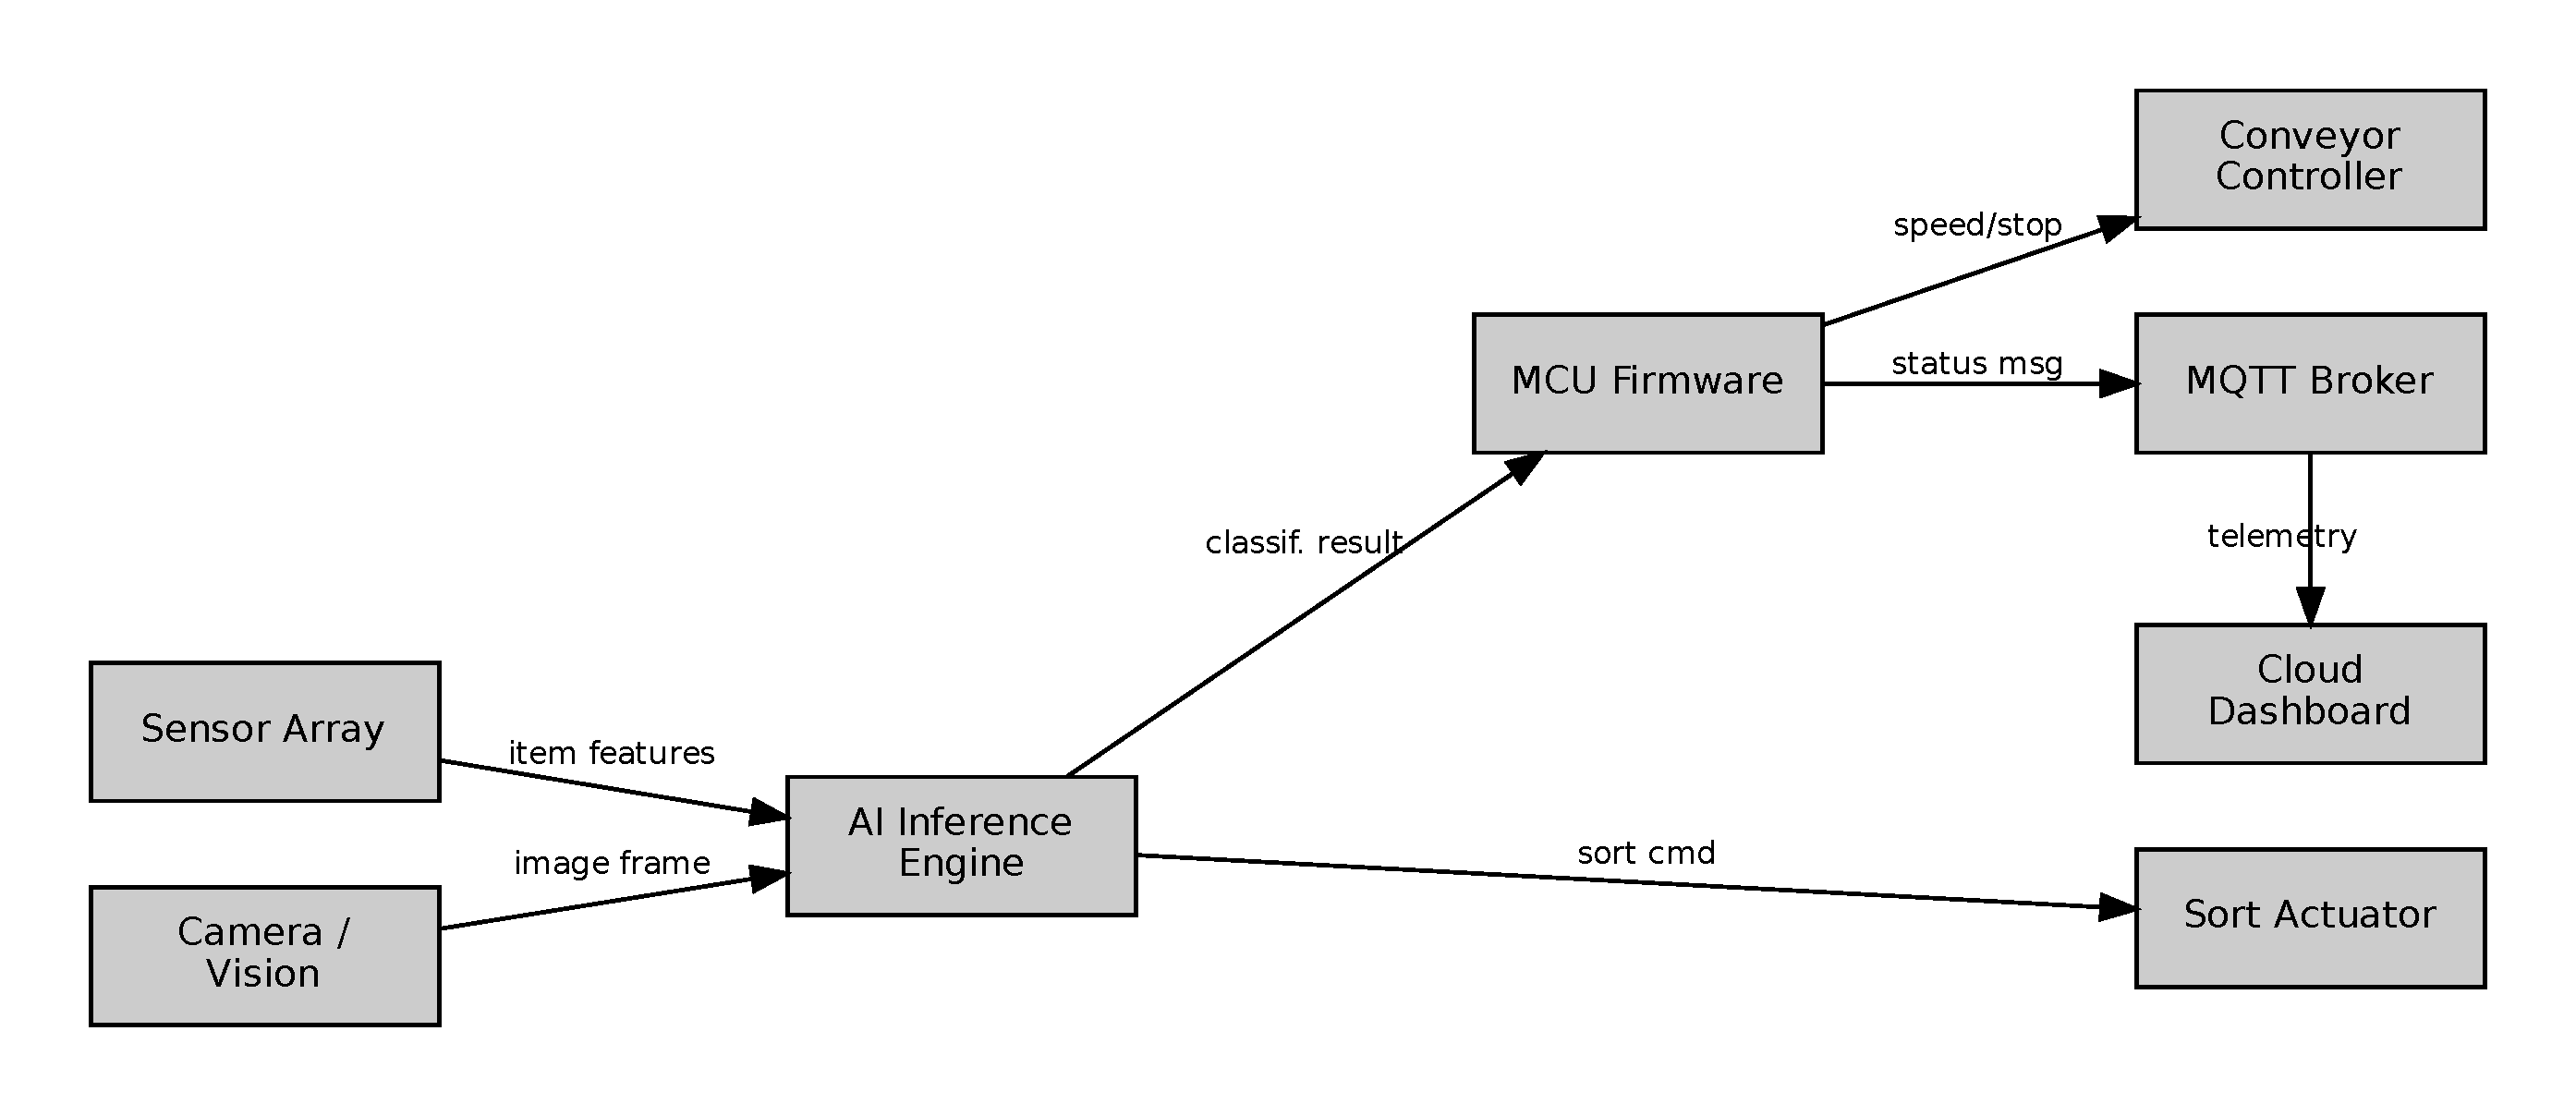
\includegraphics[width=0.88\textwidth]{images/fig_01_block_diagram}
  \caption{System block diagram for the IoT robotic sorting prototype.
           Boxes represent subsystems across the four domains; arrows represent
           interface boundaries, each of which receives a contract in
           Table~\ref{tab:ch5-interface}.
           Labels A–D correspond to the four interface types introduced in
           Section~\ref{sec:ch5-interfaces}.}
  \label{fig:ch5-block}
\end{figure}

\paragraph{In Practice.}
At the start of a team project, produce the block diagram before any other technical document.
Pin it to the shared drive or project wall.
Every team member should be able to point to their box and describe exactly what enters and exits it.
A one-page interface table built from this diagram is the single most effective tool for keeping all team members building to the same specification.
When everyone can see the same table, ``I assumed it would be 3.3~V'' is no longer a valid explanation for a three-day debugging sprint.

\paragraph{Common Pitfalls.}
\begin{itemize}
  \item \textbf{Starting the interesting subsystem before interfaces are fixed.}
        Firmware and AI engineers are often eager to write code before the electrical interfaces are settled.
        If the UART voltage level has not been agreed upon, any firmware written against an assumed level may be wrong, and the rework cost is real schedule time.
  \item \textbf{Treating the block diagram as decoration.}
        A block diagram that lives in a report appendix and is never referenced during build is not doing its job.
        It must be a living, binding contract --- updated any time a subsystem boundary changes, and consulted before any interface-crossing code or hardware is designed.
  \item \textbf{Verbal interface agreements.}
        ``We'll figure out the data format later'' is not an interface definition.
        The team that built the firmware and the team that built the AI classifier will make different assumptions, and those assumptions will collide at integration.
\end{itemize}

% ─────────────────────────────────────────────────────────────────────────────
\section{Interfaces as Contracts}
\label{sec:ch5-interfaces}
% ─────────────────────────────────────────────────────────────────────────────

An \textbf{interface}\index{interface} is the shared boundary between two subsystems.
At that boundary one subsystem makes a promise to another.
Calling it a \textbf{interface contract}\index{interface contract} is deliberate: both sides are obligated.
The provider subsystem must deliver exactly what is specified; the consumer subsystem must not demand anything beyond what is specified.
When the contract is written down, a violation is detectable.
When the contract lives only in someone's head, it is invisible until the two subsystems meet on the bench.

There are four interface types used throughout this course.
Each type has a different set of properties that must be specified to make the contract complete.

\subsection{Electrical Interfaces}
\label{subsec:ch5-elec-interface}

An \textbf{electrical interface}\index{electrical interface} specifies:
\begin{itemize}
  \item \textbf{Voltage level:} logic-high and logic-low thresholds (e.g., 3.3~V CMOS or 5~V TTL).
  \item \textbf{Current capacity:} the maximum source/sink current the provider can supply and the maximum the consumer may draw.
  \item \textbf{Protocol:} the communication standard (UART, SPI, I\textsuperscript{2}C, PWM, analog 0--5~V).
  \item \textbf{Connector:} physical connector type and pinout so that the mating is unambiguous.
  \item \textbf{Protection:} ESD handling, over-current limiting, or level-shifting requirements.
\end{itemize}

For the running-example sorter, the interface between the MCU and the motor driver is an electrical interface: 3.3~V PWM out from the MCU, 5~V logic input on the motor driver, requiring a level-shifter.
Specifying the level-shifter requirement at architecture time --- rather than discovering the incompatibility at bench time --- is the direct return on investment for this chapter's work.

\subsection{Mechanical Interfaces}
\label{subsec:ch5-mech-interface}

A \textbf{mechanical interface}\index{mechanical interface} specifies:
\begin{itemize}
  \item \textbf{Mounting geometry:} hole pattern, spacing, and tolerances.
  \item \textbf{Physical envelope:} maximum bounding box or keep-out volume.
  \item \textbf{Force or torque limits:} the maximum load the mating structure must carry.
  \item \textbf{Material compatibility:} relevant where corrosion, heat, or vibration is a factor.
\end{itemize}

For the running-example sorter, the mechanical interface between the sensor bracket and the conveyor frame defines the exact standoff height at which the time-of-flight sensor must sit relative to the belt surface.
If the firmware team writes their detection algorithm assuming a 150~mm standoff but the mechanical team fabricates a 200~mm bracket, the item-detection gate geometry is wrong and every downstream timing calculation inherits that error.

\subsection{Data Interfaces}
\label{subsec:ch5-data-interface}

A \textbf{data interface}\index{data interface} specifies:
\begin{itemize}
  \item \textbf{Protocol and transport:} MQTT, HTTP, I\textsuperscript{2}C register map, SPI frame format, serial byte stream.
  \item \textbf{Message format:} field names, data types, units, and byte order.
  \item \textbf{Topic or address:} MQTT topic string, I\textsuperscript{2}C device address, REST endpoint.
  \item \textbf{Quality of Service (QoS):} for MQTT, the QoS level (0, 1, or 2) and retained-message flag.
  \item \textbf{Error handling:} what happens if a message is lost, malformed, or arrives out of order.
\end{itemize}

For the running-example sorter, the data interface between the MCU firmware and the cloud dashboard is an MQTT publish on topic \texttt{sorter/status} with a JSON payload containing \texttt{item\_class}, \texttt{sort\_result}, and \texttt{timestamp\_ms}.
Any team member building the dashboard must consume exactly that format; any firmware update that renames a field without updating the interface table breaks the contract.

\subsection{Timing Interfaces}
\label{subsec:ch5-timing-interface}

A \textbf{timing interface}\index{timing interface} specifies:
\begin{itemize}
  \item \textbf{Latency:} the maximum time between a trigger event and the expected response.
  \item \textbf{Throughput:} the maximum number of events per second the interface must sustain.
  \item \textbf{Jitter:} the maximum variation in latency from one cycle to the next.
  \item \textbf{Deadline type:} hard (a missed deadline is a system failure), firm (a missed deadline degrades output quality), or soft (a missed deadline is acceptable occasionally).
\end{itemize}

For the running-example sorter, the timing interface between the sensor read and the AI classifier is: sensor output available within $t_1 \leq 1$~ms of item detection, with jitter $\leq 0.1$~ms.
The AI classifier must begin its inference within that window to keep the 5~ms pipeline budget intact.

\subsection{The Interface Table}
\label{subsec:ch5-interface-table}

All four interface types are collected into a single \textbf{interface table}\index{interface table} --- one row per arrow in the block diagram.
Table~\ref{tab:ch5-interface} shows the interface table for the running-example sorter.
This table is the primary deliverable of this chapter and must be completed before any subsystem build begins.

\begin{table}[htbp]
  \centering
  \caption{Interface table for the IoT robotic sorting prototype.
           Each row names a boundary from Figure~\ref{fig:ch5-block},
           its type, the contract properties, and the timing allocation
           from Section~\ref{sec:ch5-budgets}.}
  \label{tab:ch5-interface}
  \small
  \begin{tabular}{lllp{5.5cm}r}
    \hline
    \textbf{ID} & \textbf{From} & \textbf{To} & \textbf{Contract (key properties)} & \textbf{Latency} \\
    \hline
    A & Sensor & Firmware & Electrical: 3.3~V I\textsuperscript{2}C, 400~kHz; range reading in 2-byte register; detection interrupt on GPIO & $t_1 \leq 1$~ms \\
    B & Firmware & AI Engine & Data: shared memory frame buffer; 320$\times$240 px RGB888; semaphore handshake & $t_2 \leq 2$~ms \\
    C & AI Engine & Firmware & Data: classification label (uint8) + confidence (float32); written to result register; sets done flag & included in $t_2$ \\
    D & Firmware & Motor Driver & Electrical: 3.3~V PWM $\to$ level-shifted 5~V; direction GPIO; 20~kHz carrier & $t_3 \leq 2$~ms \\
    E & Firmware & MQTT Broker & Data: TCP/IP; topic \texttt{sorter/status}; JSON payload; QoS~1; $\leq$200~ms publish latency & async \\
    F & Sensor Bracket & Conveyor Frame & Mechanical: M3 $\times$ 4-hole pattern, 20~mm spacing; standoff $150 \pm 2$~mm; max load 0.5~N & N/A \\
    \hline
  \end{tabular}
\end{table}

% ─────────────────────────────────────────────────────────────────────────────
\section{Budget Allocation}
\label{sec:ch5-budgets}
% ─────────────────────────────────────────────────────────────────────────────

Specifying interfaces is necessary but not sufficient.
You must also verify that the sum of all subsystem demands does not exceed the system-level constraint.
This verification is called \textbf{budget allocation}\index{budget allocation}: you divide a finite resource --- time, power, or permissible error --- across the subsystems that consume it, and then confirm the total stays within the specification limit.

Three budgets matter for the running-example prototype: timing, power, and measurement error.

\subsection{Timing Budget}
\label{subsec:ch5-timing-budget}

The \textbf{timing budget}\index{timing budget} formalises the constraint that the sum of all pipeline-stage latencies must not exceed the specification deadline.

\begin{equation}
  T_{\text{total}} = \sum_{i} t_i \leq T_{\text{budget}}
  \label{eq:ch5-timing}
\end{equation}

This is the budget structure introduced in Chapter~4's risk analysis (Equation~\ref{eq:ch4-budget-sum}).
Here it is stated formally as the governing inequality for the architecture.
Every timing interface in the interface table must carry a $t_i$ allocation; those allocations are substituted into Equation~\ref{eq:ch5-timing} to verify the total.

\subsection{Power Budget}
\label{subsec:ch5-power-budget}

The \textbf{power budget}\index{power budget} verifies that the supply rail can deliver enough current for all subsystems simultaneously.

\begin{equation}
  P_{\text{total}} = \sum_{i} P_i
  \label{eq:ch5-power}
\end{equation}

$P_{\text{total}}$ must not exceed the rated output of the power supply.
For the running-example sorter on a 5~V/2~A USB supply (10~W), typical subsystem allocations are: MCU 0.5~W, camera module 1.2~W, motor driver (idle) 0.8~W, motor driver (active) 2.5~W, Wi-Fi module 0.9~W --- a peak total of 5.9~W, well within the 10~W budget with a 4.1~W margin.
Margins matter: a motor driver that draws more than rated, a Wi-Fi transmit burst that spikes current, or a future addition of an LED indicator can each erode headroom.
Figure~\ref{fig:ch5-budget} shows the timing and power budgets as stacked bars against their respective limit lines.

\begin{figure}[htbp]
  \centering
  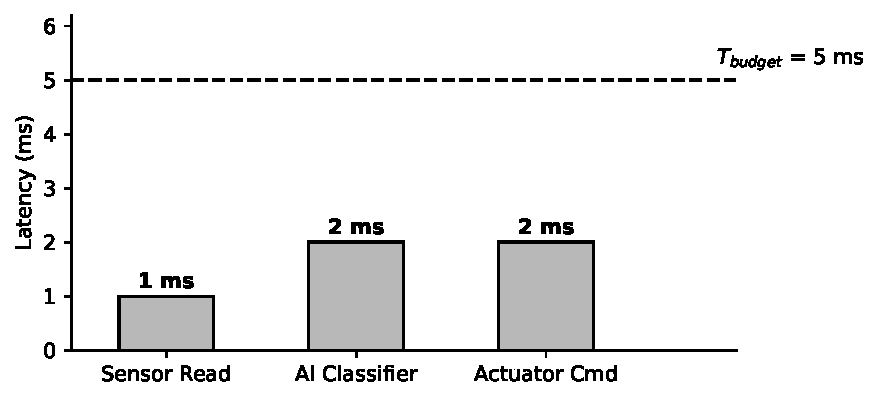
\includegraphics[width=0.85\textwidth]{images/fig_02_interface_budget}
  \caption{Interface budgets for the running-example sorter.
           Left panel: timing budget --- stacked bar of $t_1$, $t_2$, $t_3$
           against the 5~ms limit line (Equation~\ref{eq:ch5-timing}).
           Right panel: power budget --- stacked bar of subsystem power
           draws against the 10~W supply limit (Equation~\ref{eq:ch5-power}).
           Zero margin on timing means any added pipeline step requires removing
           an existing one.}
  \label{fig:ch5-budget}
\end{figure}

\subsection{Error Budget}
\label{subsec:ch5-error-budget}

Multiple measurement stages each contribute their own uncertainty.
Assuming the error sources are independent and random, they combine in \textbf{quadrature}\index{root-sum-of-squares error} (root-sum-of-squares, RSS):

\begin{equation}
  e_{\text{total}} = \sqrt{\sum_{i} e_i^{\,2}}
  \label{eq:ch5-rss}
\end{equation}

The RSS model is more realistic than a worst-case linear sum because independent errors partially cancel.
If $e_{\text{total}}$ exceeds the acceptance criterion, the team must tighten the largest individual contributor first --- squeezing a small contributor yields almost no benefit once a dominant error source exists.

\subsection{Worked Example --- Part A: Timing Budget}
\label{subsec:ch5-worked-timing}

The central question from Chapter~3 requires classifying and diverting each item within $\leq$167~ms of arrival (6~items/min), but the firmware pipeline latency must be far shorter so that the MQTT publish and mechanical diversion can complete within that window.
Chapter~4's risk analysis established a firmware timing budget of $T_{\text{budget}} = 5$~ms with three pipeline stages.
Applying Equation~\ref{eq:ch5-timing}:

\[
  T_{\text{total}} = t_1 + t_2 + t_3 = 1\text{ ms} + 2\text{ ms} + 2\text{ ms} = 5\text{ ms}
\]

\[
  T_{\text{total}} = 5\text{ ms} \leq T_{\text{budget}} = 5\text{ ms} \quad \checkmark
\]

\noindent where:
\begin{itemize}
  \item $t_1 = 1$~ms: sensor read (I\textsuperscript{2}C transaction, distance measurement, interrupt service);
  \item $t_2 = 2$~ms: AI classifier inference (image capture, pre-processing, forward pass, label decode);
  \item $t_3 = 2$~ms: actuator command (PWM update, GPIO direction set, motor driver settling).
\end{itemize}

The budget passes, but the \textbf{dwell-time margin is zero}.
Any added pipeline step --- a second sensor read for confirmation, a logging write to flash, a display update --- requires shortening one of the existing stages by an equal amount.
This constraint must be visible to every team member: firmware engineers do not add steps to this pipeline without a corresponding timing analysis showing where the recovered time comes from.

\subsection{Worked Example --- Part B: RSS Error Budget}
\label{subsec:ch5-worked-rss}

The sort-accuracy specification requires $\geq$95\% classification accuracy.
Three independent sources of measurement uncertainty contribute to positional error at the classification gate:

\begin{itemize}
  \item $e_1 = \pm 0.05$~m/s: conveyor speed sensor uncertainty, which introduces positional error when the system computes item position from belt velocity.
        At the nominal belt speed of $0.05$~m/s, a speed uncertainty of $\pm 0.05$~m/s maps to a relative positional uncertainty of $\pm(0.05/0.05)\times 1\% = \pm 0.1\%$; this is the value substituted as $e_1$ in the RSS calculation.
  \item $e_2 = \pm 0.5\%$: AI vision classification uncertainty (probability gap between top-1 and top-2 class, expressed as a percentage-point uncertainty in the sort decision).
  \item $e_3 = \pm 0.3\%$: positional uncertainty equivalent derived from timing jitter of $\pm 0.1$~ms mapped through the nominal belt speed.
\end{itemize}

Expressing all contributors in compatible units (percentage-point equivalent positional uncertainty) and applying Equation~\ref{eq:ch5-rss}:

\noindent $e_1 = 0.1\%$, $e_2 = 0.5\%$, $e_3 = 0.3\%$

\[
  e_{\text{total}} = \sqrt{(0.1\%)^2 + (0.5\%)^2 + (0.3\%)^2}
  = \sqrt{0.01 + 0.25 + 0.09}\%
  = \sqrt{0.35}\%
  \approx 0.59\%
\]

The acceptance criterion is $e_{\text{total}} \leq 0.6\%$.

\[
  e_{\text{total}} \approx 0.59\% \leq 0.60\% \quad \checkmark
\]

The error budget passes --- but barely.
The dominant contributor is $e_2$, the AI classification uncertainty.
If the model's confidence gap narrows (e.g., the item class becomes harder to distinguish), this budget will fail at that contributor first.
Chapter~6 will revisit this when selecting the camera sensor and AI model architecture.

\paragraph{In Practice.}
A team building a motor controller prototype skipped the electrical interface table and started firmware before agreeing on the UART voltage level between the MCU and the motor driver.
The MCU operated at 3.3~V logic; the motor driver expected 5~V logic.
The firmware team wrote and tested their UART code against a bench logic analyser at 3.3~V.
The electronics team wired the motor driver directly to the MCU TX pin.
At integration, the motor driver received marginal logic levels: it sometimes responded and sometimes did not, depending on supply current at the moment of the transaction.
Diagnosing the intermittent fault cost three days.
The fix was a single-chip level-shifter --- a \$0.30~CAD part that would have taken ten minutes to add to the schematic during architecture definition.
The interface table entry for that boundary would have read: \emph{``Electrical: MCU UART TX at 3.3~V CMOS logic; motor driver UART RX requires 5~V TTL; level-shifter required on this net.''}
Three days of debugging for a \$0.30 part and one table row.

% ─────────────────────────────────────────────────────────────────────────────
\section{Why Integration Fails at Boundaries}
\label{sec:ch5-failures}
% ─────────────────────────────────────────────────────────────────────────────

\index{integration failure}Subsystems fail at their boundaries, not at their centres.
This statement is almost universally true in mechatronic and embedded prototype development, and it has a straightforward explanation.

Within a subsystem, one engineer (or one small team) controls all the assumptions.
The firmware engineer who writes the sensor driver and the interrupt handler is working within a single, consistent mental model.
The mechanical engineer who designs the conveyor frame is making choices within their own constraints.
Bugs within a subsystem are caught during subsystem-level testing because the developer is testing exactly the thing they understand.

At a boundary, two or more parties each independently assumed something about the other's subsystem.
Those assumptions were never formally compared.
When the two subsystems meet for the first time, every mismatched assumption becomes a defect.
Figure~\ref{fig:ch5-boundary} illustrates a canonical boundary mismatch: two subsystems whose interface contracts were never formally aligned, resulting in an incompatible handshake at integration.

\begin{figure}[htbp]
  \centering
  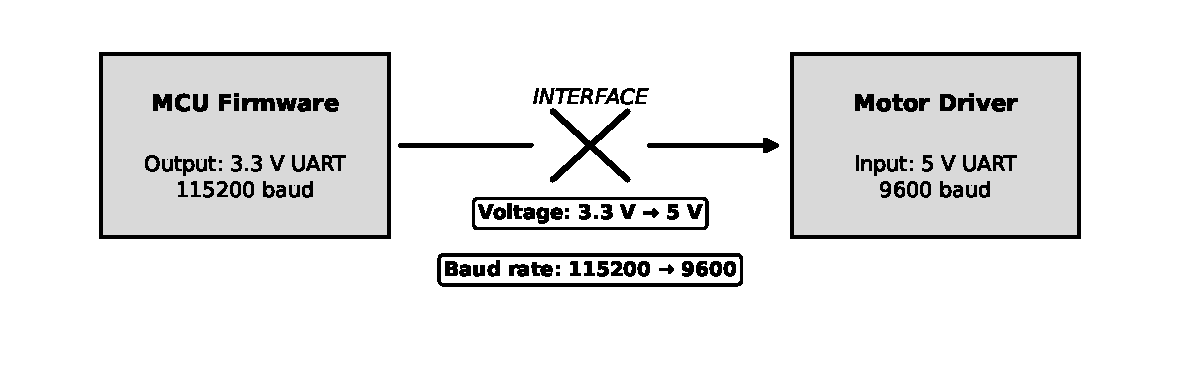
\includegraphics[width=0.78\textwidth]{images/fig_03_boundary_failure}
  \caption{Boundary mismatch at integration.
           The left subsystem (MCU firmware) assumes 3.3~V CMOS logic and
           outputs a valid signal by its own standard; the right subsystem
           (motor driver) expects 5~V TTL and interprets the same signal as
           an indeterminate logic level.
           Neither subsystem contains a bug in isolation; the defect exists
           only at the boundary, and is invisible until the two are connected.}
  \label{fig:ch5-boundary}
\end{figure}

\subsection{Taxonomy of Boundary Failures}
\label{subsec:ch5-boundary-types}

Four categories of boundary failure recur across student and professional projects alike.

\subsubsection{Voltage Level Mismatch}
\label{subsubsec:ch5-voltage-mismatch}

\index{voltage level mismatch}The most common electrical boundary failure: one subsystem drives 3.3~V logic, the adjacent subsystem expects 5~V, and neither team checked the other's datasheet.
Outcome: intermittent communication, latent damage to 3.3~V pins exposed to 5~V, or total non-function.
Prevention: one row in the electrical interface table, one level-shifter on the BOM.

\subsubsection{Protocol Mismatch}
\label{subsubsec:ch5-protocol-mismatch}

\index{protocol mismatch}One subsystem writes a SPI frame formatted as 16-bit big-endian; the consuming subsystem reads it as 16-bit little-endian.
Both subsystems pass their individual unit tests.
The integration test produces garbage output that takes hours to trace to a byte-order disagreement.
Prevention: specify byte order, data type, and endianness in the data interface contract.

\subsubsection{Timing Assumption Mismatch}
\label{subsubsec:ch5-timing-mismatch}

\index{timing assumption mismatch}The firmware team assumes the AI engine returns a result within 2~ms.
The AI team benchmarks their model at 3~ms on the prototype hardware.
The pipeline budget fails by 1~ms and the diverter fires 1~ms after the item has already passed the gate.
Prevention: the timing interface contract specifies the maximum latency; the AI team runs a benchmark on the actual target hardware and signs off before build begins.

\subsubsection{Mechanical Fit Mismatch}
\label{subsubsec:ch5-mechanical-mismatch}

\index{mechanical fit mismatch}The sensor bracket is designed for a sensor with an M2.5 mounting hole.
The sensor that arrives has an M3 mounting hole.
Fabrication is already complete.
Prevention: the mechanical interface contract specifies the exact hole pattern, fastener size, and tolerance, and is verified against the component datasheet before fabrication is released.

\subsection{Identifying the Highest-Risk Boundary}
\label{subsec:ch5-highest-risk}

Not all boundaries carry equal risk.
The boundary with the highest integration risk is the one where:
\begin{enumerate}
  \item the two subsystems are developed by different people or teams with limited communication;
  \item the interface contract is the least precisely specified; and
  \item a mismatch at this boundary would be the hardest to detect before it causes visible system failure.
\end{enumerate}

This is precisely the FMEA detection factor $D$ from Chapter~4 applied at the interface level.
For the running-example sorter, the firmware-to-AI-engine boundary (Interface~B in Table~\ref{tab:ch5-interface}) carries the highest integration risk: the shared memory frame buffer protocol is non-standard, the two subsystems may be developed on different toolchains, and a timing assumption mismatch here propagates directly into a missed divert-gate deadline.

\paragraph{Common Pitfalls.}
\begin{itemize}
  \item \textbf{``We'll figure it out later'' interface agreements.}
        Verbal agreements about data formats, voltage levels, or timing are not interface contracts.
        They are deferred arguments.
        Experienced engineers know that ``later'' always arrives during integration, when schedule pressure is highest and the cost of rework is greatest.
  \item \textbf{Developing the interesting subsystem first.}
        AI engineers naturally want to train and test the classifier.
        Firmware engineers want to write drivers.
        Without fixed interfaces, each group builds to their own internally consistent assumptions, and integration becomes a negotiation between two finished products that were never designed to meet each other.
  \item \textbf{Interface table as a compliance artifact.}
        Filling out the interface table to satisfy a deliverable requirement, then ignoring it during build, defeats its purpose.
        The table must be the reference document that every team member checks before crossing a subsystem boundary.
\end{itemize}

% ─────────────────────────────────────────────────────────────────────────────
\subsection*{Try It Yourself}
\label{sec:ch5-tiy}
% ─────────────────────────────────────────────────────────────────────────────

\textbf{Scenario:} You are architecting a wireless air-quality monitor.
The specification requires a total firmware pipeline latency of $T_{\text{budget}} = 8$~ms.
Three pipeline stages have been proposed:
\begin{itemize}
  \item $t_1 = 2$~ms: ADC sample (sensor read and digitisation);
  \item $t_2 = 3$~ms: digital filter (moving-average computation on the MCU);
  \item $t_3 = 2$~ms: BLE transmit buffer (packetise reading and push to BLE stack).
\end{itemize}

Three measurement error sources contribute to the reported air-quality reading:
\begin{itemize}
  \item $e_1 = \pm 0.3$\textdegree{}C equivalent: temperature sensor uncertainty;
  \item $e_2 = \pm 1.5$\textdegree{}C equivalent: humidity sensor uncertainty (the \%~RH specification has been pre-converted to a temperature-equivalent for this budget);
  \item $e_3 = \pm 0.1$\textdegree{}C equivalent: ADC quantization noise.
\end{itemize}

The acceptance criterion for the combined error is $e_{\text{total}} \leq 1.6$\textdegree{}C equivalent.

\bigskip
\noindent\textbf{Tasks:}

\begin{enumerate}
  \item[(a)] \textbf{Timing budget.}
        Using Equation~\ref{eq:ch5-timing}, compute $T_{\text{total}} = t_1 + t_2 + t_3$.
        State whether the timing budget is satisfied and identify the remaining margin (if any).

  \item[(b)] \textbf{Error budget.}
        Using Equation~\ref{eq:ch5-rss}, compute $e_{\text{total}}$ from the three error sources.
        State whether the error budget passes the acceptance criterion and identify the dominant contributor.

  \item[(c)] \textbf{Constraint violation response.}
        If the firmware team's digital filter implementation turns out to require $t_2 = 4$~ms instead of 3~ms, $T_{\text{total}}$ will exceed $T_{\text{budget}}$.
        Identify which stage(s) could be shortened to restore compliance.
        For each option you propose, state the new $t_i$ value and verify that the revised $T_{\text{total}} \leq 8$~ms.

  \item[(d)] \textbf{Interface contract.}
        Identify one interface in this air-quality monitor system (choose a boundary you consider the highest integration risk).
        Write a two-line interface contract for that boundary, specifying: (line 1) the protocol and voltage level or data format; (line 2) the timing constraint.
\end{enumerate}

% ─────────────────────────────────────────────────────────────────────────────
\section*{Review Questions}
\label{sec:ch5-review}
% ─────────────────────────────────────────────────────────────────────────────

\begin{enumerate}

  \item \textbf{(Conceptual)} State the four interface types defined in this chapter.
        For each type, give one specific example from the running-example IoT sorter system, naming the two subsystems at the boundary and one key property of the contract.

  \item \textbf{(Conceptual)} Explain in two sentences why integration bugs typically appear at boundaries between subsystems rather than within a subsystem.
        Your answer should reference the concept of locally consistent assumptions within a subsystem versus the unverified assumptions that cross a boundary.

  \item \textbf{(Conceptual --- classification)} A team proposes an interface between the MCU and a Bluetooth module described only as ``send the JSON string over serial.'' Classify the completeness of this interface contract: state which of the four interface types it partially addresses, which required properties are missing, and explain why the omissions constitute integration risk.

  \item \textbf{(Applied --- calculation)}
        A firmware pipeline has four stages with the following latency allocations:
        $t_1 = 0.8$~ms, $t_2 = 1.2$~ms, $t_3 = 0.6$~ms, $t_4 = 0.9$~ms.
        The timing specification requires $T_{\text{budget}} = 4$~ms.
        \begin{enumerate}
          \item Compute $T_{\text{total}}$ using Equation~\ref{eq:ch5-timing}.
          \item State whether the timing budget is satisfied.
                If it is satisfied, state the margin.
          \item An added 0.8~ms logging step is required. How must the existing stage allocations be adjusted to keep $T_{\text{total}} \leq 4$~ms? State which stage(s) to shorten and by how much.
        \end{enumerate}

  \item \textbf{(Applied --- multi-step)}
        Three subsystems each contribute independent positional measurement error to a parts-placement robot:
        encoder $e_1 = \pm 0.2$~mm, vision sensor $e_2 = \pm 0.5$~mm, synchronisation jitter equivalent $e_3 = \pm 0.1$~mm.
        The acceptance criterion is $e_{\text{total}} \leq 0.7$~mm.
        \begin{enumerate}
          \item Compute $e_{\text{total}}$ using Equation~\ref{eq:ch5-rss}.
                Show all intermediate steps.
          \item State whether the error budget passes the acceptance criterion.
                If it passes, state the margin; if it fails, state the deficit.
          \item The vision sensor is upgraded to a model with $\pm 0.3$~mm uncertainty.
                Recompute $e_{\text{total}}$ and state the new margin against the 0.7~mm criterion.
        \end{enumerate}

\end{enumerate}

% ─────────────────────────────────────────────────────────────────────────────
\subsection*{End-of-Chapter Artifact}
\label{sec:ch5-artifact}
% ─────────────────────────────────────────────────────────────────────────────

By the end of this chapter your project folder must contain one deliverable:

\medskip
\noindent\textbf{System Architecture Package:} the system block diagram (Figure~\ref{fig:ch5-block}) plus a completed interface table with every subsystem boundary from that diagram named, its four-property contract defined, and the timing and power budget columns filled in and verified against Equations~\ref{eq:ch5-timing} and~\ref{eq:ch5-power}.

\medskip
Specifically, the package must demonstrate:
\begin{itemize}
  \item A labelled block diagram with one box per subsystem across the four domains (electronics, mechanical, firmware, AI/IoT/robotic logic) and one labelled arrow per interface.
  \item An interface table in which each row names the two subsystems at the boundary, states the interface type (electrical, mechanical, data, or timing), and specifies the key contract properties.
  \item A timing budget column showing $t_i$ allocations that sum to $T_{\text{total}} \leq T_{\text{budget}}$ (Equation~\ref{eq:ch5-timing}).
  \item A power budget column showing $P_i$ allocations that sum to $P_{\text{total}}$ (Equation~\ref{eq:ch5-power}), with the total compared to the rated supply output.
  \item A written identification of the highest-risk boundary, with a two-sentence justification referencing the interface type and the detection difficulty of a mismatch at that boundary.
\end{itemize}

The block diagram and completed interface table together form the \textbf{Gate~3 architecture deliverable} (see the Stage-Gate model established in Chapter~2).
A Gate~3 reviewer will verify: (1)~every arrow in the block diagram has a corresponding row in the interface table; (2)~each row carries a complete four-property contract; and (3)~the timing and power budget columns close against Equations~\ref{eq:ch5-timing} and~\ref{eq:ch5-power}.
A package that fails any of these three checks does not satisfy the Gate~3 architecture criterion.

% ─────────────────────────────────────────────────────────────────────────────
\section*{Chapter Summary}
\label{sec:ch5-summary}
% ─────────────────────────────────────────────────────────────────────────────

Three tools now equip you to move from specification to buildable architecture.

First, a \textbf{decomposition framework}: dividing any prototype into four subsystem domains --- electronics, mechanical, firmware, and AI/IoT/robotic logic --- gives every team member an unambiguous scope and transforms integration from a surprise into a managed handshake.

Second, a \textbf{contract language for interfaces}: every boundary between subsystems carries a formal contract specifying electrical properties, mechanical geometry, data format, and timing constraints.
A boundary without a contract is a liability that will be paid at integration time.
The interface table is the instrument that makes all contracts visible to the whole team simultaneously.

Third, a \textbf{budget discipline}: timing, power, and measurement error are finite resources.
Equations~\ref{eq:ch5-timing}, \ref{eq:ch5-power}, and~\ref{eq:ch5-rss} provide the arithmetic to verify that the sum of subsystem demands fits within the system-level limits.
For the running-example sorter, the 5~ms timing budget is exactly consumed by the three pipeline stages, leaving zero margin; the power budget carries a 4.1~W margin; and the RSS error budget passes the 0.6\% criterion by the narrowest of margins, flagging AI classification uncertainty as the risk to watch.

The architecture established here is the foundation on which Chapter~6 builds: the System Architecture Package gives Chapter~6 its starting point, and every component selected there will be evaluated against the interface contracts written here.
